50. \begin{figure}[ht!]
\center{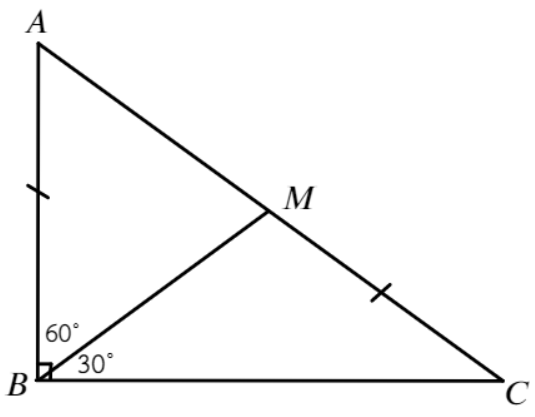
\includegraphics[scale=0.35]{g9-49.png}}
\end{figure}\\
Из теорем синусов для треугольников $AMB$ и $CMB$ получим равенства\\ $\cfrac{AB}{\sin(AMB)}=\cfrac{AM}{\sin(60^\circ)},\ \cfrac{BC}{\sin(\angle BMC)}= \cfrac{MC}{\sin(30^\circ)}.$ Так как синусы смежных углов равны, после деления равенств друг на друга получим соотношение $\cfrac{AB}{BC}=\cfrac{AM\cdot\cfrac{1}{2}}{MC\cdot\cfrac{\sqrt{3}}{2}},$ откуда $AM\cdot BC=9\sqrt{3}.$ Пусть $BC=x,$ тогда $AM=\cfrac{9\sqrt{3}}{x}.$ По теореме Пифагора имеем $x^2+9=\left(\cfrac{9\sqrt{3}}{x}+3
ight)^2,\ x^2+9=\cfrac{243}{x^2}+\cfrac{54\sqrt{3}}{x}+9,\ x^4-54\sqrt{3}x-243=0,\ x^4-3\sqrt{3}x^3+3\sqrt{3}x^3-27x^2+27x^2-81\sqrt{3}x+27\sqrt{3}x-243=0,$\\
$x^3(x-3\sqrt{3})+3\sqrt{3}x^2(x-3\sqrt{3})+27x(x-3\sqrt{3})+27\sqrt{3}(x-3\sqrt{3})=0,\ (x-3\sqrt{3})(x^3+3\sqrt{3}x^2+27x+27\sqrt{3})=0,\ x=3\sqrt{3}$см. Решение единственно, так как $x>0.$\\
